\capitulo{5}{Aspectos relevantes del desarrollo del proyecto}

\section{Entorno de desarrollo}
Como entorno de desarrollo de los prototipos hemos designado Jupyter ya que en sus notebooks interactivos puedes ejecutar directamente código python como si fuese un interprete.\\

\subsection{Ventajas}
\begin{itemize}
\item He podido añadir widguets para calibrar en buen grado las funciones que hemos utilizado.\\
Gracias a estos widguets podemos dar valores e ir viendo como cambia la salida de la función de forma interactiva.

\begin{figure}[h]
\centering
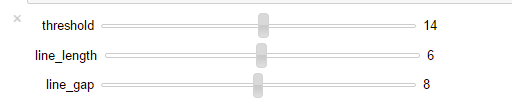
\includegraphics[scale=0.75]{Widget}
\caption{Ejemplo de un widguet sobre la función de hough}
\end{figure}

\item Su rápida visualización sin tener grandes conocimientos de interfaz gráfica ha sido un gran apoyo para poder visualizar desde el principio las imágenes procesadas y como quedaban.\\ 

\begin{figure}[h]
\centering
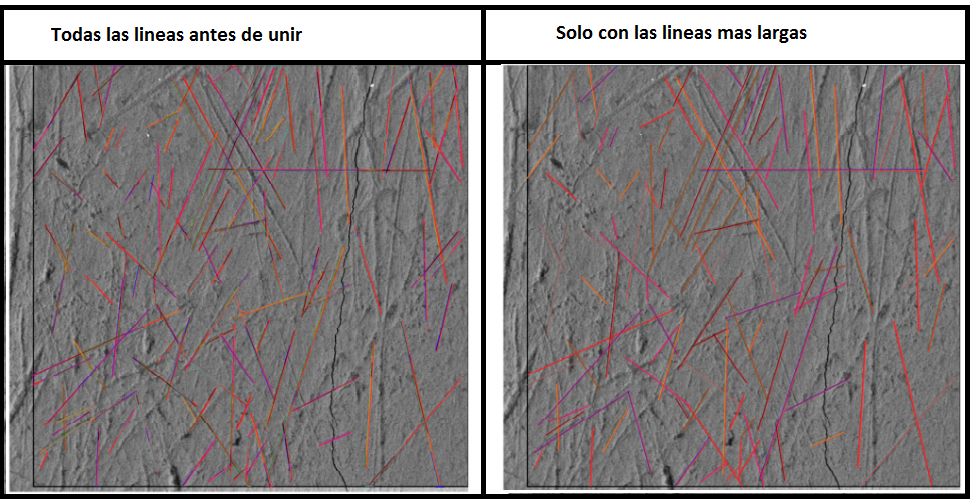
\includegraphics[scale=0.55]{ComparativaLineas}
\caption{Ejemplo de una visualización del resultado intermedio de las funciones.}
\end{figure}

\item Desde el propio entorno puedes ejecutar no solo código estructurado en script sino también código estructurado en clases y llamadas a métodos es como un IDE pero con limitaciones.

\begin{figure}[h]
\centering
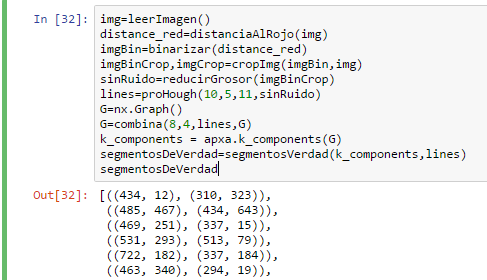
\includegraphics[scale=0.75]{Ejecucion}
\caption{Ejemplo de una Ejecución.}
\end{figure}

\item Multitud de librerías y funciones que en entornos parecidos como matlab serian de pago y aquí al ser software libre el ejemplo anterior lo resume en una librería numpy \cite{Numpy}.
\end{itemize}

\section{Procesado imagen}
Para llegar a conseguir calcular las lineas que había pintadas en las imágenes tube que realizar una serie de pasos que vamos a resumir en tres etapas.
\subsection{Binarización}
Partiendo de una imagen que solo tenia lineas en rojo pintadas encima de las estrías producidas por el desgaste y lo demás de la imagen en escala de grises, lo primero fue leer la imagen a trabes de las funciones ya programadas en la librería de Scikit-Image(skimage).\\
Una vez que tenemos la imagen guardada en el espacio de color RGB podemos empezar el procesado quedándonos con el canal Rojo.\\
Calculamos la distancia de cada pixel de la imagen al color rojo restando, uno menos el valor absoluto del pixel en el canal S (saturación) del espacio de color HSV , (restando el valor absoluto a la unidad conseguimos normalizar entre [0-1])y pasamos la imagen de distancias a blanco y negro y así tendremos un valor entre 0 y 256 en cada pixel correspondiente a la distancia al rojo cuanto mas alejado mas negro y los que sean rojos en blanco.\\
Para que la diferencia sea blanco o negro binarizamos la imagen con un valor umbral calculado como threshold otsu y así la imagen los valores de la distancia que sean mayores que el umbral pasaran a valer máximo y los que no consigan pasar el umbral serán los bordes(blanco).

\subsection{Obtener segmentos}
Partimos de la imagen binarizada y lo primero es reducir el grosor de las lineas detectadas a 1 pixel eso lo conseguimos llamando a la función skeletonize que nos devuelve la imagen con las lineas de 1 pixel (así no acumulamos errores y es mas rápida la búsqueda de rectas).\\
Seguidamente llamamos a la función "probabilistic hough line" que nos va a encontrar segmentos que formaran las lineas el funcionamiento ha sido explicado en el apartado (conceptos teóricos).

\subsection{Procesado de segmentos}
Llegados a este punto lo que tenemos son muchos segmentos que forman las lineas reales y tenemos que unirlos.\\
Para ello vamos a usar la teoría de grafos añadiendo los segmentos a un grafo.\\
Para unir dos segmentos tiene que cumplirse que la distancia mínima entre sus extremos sea menor que un umbral y si pasa este punto comprobaremos que el angulo que forman entre ellas sea menor a otro umbral y si cumplen las dos condiciones añadiremos un camino al grafo desde la recta 1 a la recta 2.
\subsection{Recuperación de lineas}
Ahora lo que tenemos es un grafo con clusters ya que cada cluster se identifica con únicamente una recta y tendremos tantos como rectas.
Un problema de grafos es el problema de las k-componentes pero a nosotros solo nos interesan las 1-componentes del grafo ya que cada grupo de estos segmentos "cercanos" se corresponde con una recta real.
devolvemos la combinación de los segmentos mas relevantes de cada cluster y estos se convierten en nuestra buscada linea real.

\subsection{Resumen pasos}

\begin{itemize}
\item Binarizar la imagen para solo quedarnos con los objetos de interés
\item Obtener segmentos que forman trozos de las lineas.
\item Añadir caminos entre las lineas cercanas en un grafo
\item obtener los grupos de lineas próximas y devolver la recta que las una. 
\end{itemize}


%Este apartado pretende recoger los aspectos más interesantes del desarrollo del %proyecto, comentados por los autores del mismo.
%Debe incluir desde la exposición del ciclo de vida utilizado, hasta los %detalles de mayor relevancia de las fases de análisis, diseño e implementación.
%Se busca que no sea una mera operación de copiar y pegar diagramas y extractos %del código fuente, sino que realmente se justifiquen los caminos de solución %que se han tomado, especialmente aquellos que no sean triviales.
%Puede ser el lugar más adecuado para documentar los aspectos más interesantes %del diseño y de la implementación, con un mayor hincapié en aspectos tales como %el tipo de arquitectura elegido, los índices de las tablas de la base de datos, %normalización y desnormalización, distribución en ficheros3, reglas de negocio %dentro de las bases de datos (EDVHV GH GDWRV DFWLYDV), aspectos de desarrollo %relacionados con el WWW...
%Este apartado, debe convertirse en el resumen de la experiencia práctica del %proyecto, y por sí mismo justifica que la memoria se convierta en un documento %útil, fuente de referencia para los autores, los tutores y futuros alumnos.
